\documentclass[a4paper,conference]{IEEEtran}

\usepackage{ifpdf}
\usepackage{cite}
\usepackage[pdftex]{graphicx}
\usepackage{array}
\usepackage{mdwmath}
\usepackage{mdwtab}
\usepackage{amssymb,latexsym}
\usepackage{stfloats}
\usepackage{amsmath}
\usepackage{subfig}
\usepackage{algcompatible}
\usepackage{algorithm}
\usepackage[font={footnotesize}]{caption}
\usepackage{balance}
\usepackage[utf8]{inputenc}
\usepackage[T1]{fontenc}
\usepackage[compatible]{algpseudocode}
\renewcommand{\figurename}{Figure}

\DeclareRobustCommand*{\IEEEauthorrefmark}[1]{%
\raisebox{0pt}[0pt][0pt]{\textsuperscript{\footnotesize\ensuremath{#1}}}}
\renewcommand\IEEEkeywordsname{Keywords}
\renewcommand{\citedash}{--}
\captionsetup{labelsep=period}

\makeatletter
\setlength{\footskip}{20pt}
\def\ps@IEEEtitlepagestyle{%
  \def\@oddfoot{\mycopyrightnotice}%
  \def\@evenfoot{}%
}
\def\mycopyrightnotice{%
  {\footnotesize Appropriate copyright notice to be put here in camera-ready version.\hfill}%
  \gdef\mycopyrightnotice{}%
}
\makeatother

\begin{document}

\title{Image Reconstruction Using the Expectation-Maximization Algorithm with 2D Gaussian Mixtures}

\author{\IEEEauthorblockN{
Martin Hornáček\IEEEauthorrefmark{1},
Radoslav Vargic\IEEEauthorrefmark{1},
Gregor Rozinaj\IEEEauthorrefmark{1}}
\IEEEauthorblockA{\IEEEauthorrefmark{1}
Faculty of Electrical Engineering and Information Technology\\
Slovak University of Technology in Bratislava\\
Ilkovičova 3, 841 04 Bratislava, Slovakia\\
{\it martin.hornacek@stuba.sk} \quad {\it radoslav.vargic@stuba.sk} \quad {\it gregor.rozinaj@stuba.sk}}}

\maketitle

\begin{abstract}
Gaussian Splatting has established the effectiveness of 2D Gaussian primitives
for image representation.
In this paper we revisit this problem through the lens of the
Expectation-Maximization (EM) algorithm for Gaussian Mixture Models, studying
how well a fixed budget of $K$ Gaussians can reconstruct a still image without
any backpropagation or learning-rate tuning.
Each Gaussian is characterised by a 2D mean, a full covariance matrix, and an
RGB colour, yielding a compact parametric description of the image.
We further propose a tiled variant in which the image is partitioned into
non-overlapping blocks, each independently fitted with EM, enabling parallelism
and scalability to larger images.
Experiments on the Kodak PhotoCD benchmark (24 images, downscaled to
$256\!\times\!256$) show that the one-shot
EM fit achieves a mean PSNR of 20.89\,dB at $K\!=\!128$ and 23.79\,dB at
$K\!=\!1024$, while the tiled variant scales to larger Gaussian budgets, enabling higher reconstruction quality.
We additionally investigate an iterative residual-refinement scheme and find
that it does not improve upon the one-shot EM baseline, motivating future
work on gradient-based refinement.
\end{abstract}

\begin{IEEEkeywords}
Gaussian Mixture Model; Expectation-Maximization; Image Reconstruction;
Gaussian Splatting; Kodak Dataset
\end{IEEEkeywords}

\IEEEpeerreviewmaketitle

% =========================================================================
\section{Introduction}
\label{sec:intro}
% =========================================================================

3D Gaussian Splatting \cite{kerbl3Dgaussians} has attracted significant
attention as an alternative to Neural Radiance Fields (NeRFs)~\cite{mildenhall2020nerf}
for real-time novel-view synthesis.
Its success is largely attributed to the use of anisotropic 3D Gaussian
primitives that are both expressive and differentiable, enabling gradient-based
optimisation via the Adam optimizer~\cite{kingma2017adam}.

A natural question is how well the \emph{statistical} estimation
counterpart, the Expectation-Maximization (EM) algorithm for Gaussian Mixture
Models, can serve as an alternative fitting procedure for the same class of
primitives.
EM is a well-understood algorithm with guaranteed monotone likelihood
improvement~\cite{dempster1977em}, and it requires no learning rate tuning.
Studying EM in the simpler 2D setting provides insight into the representational
capacity of Gaussian mixtures and motivates hybrid schemes that combine EM
initialisation with gradient-based refinement.

In this paper we address the following question: given a fixed budget of $K$
Gaussian primitives, how accurately can a 2D image be reconstructed using EM,
and what gains are possible via iterative residual refinement?
Our contributions are:
\begin{enumerate}
  \item A 2D image reconstruction pipeline based on GMM fitting with the EM
        algorithm, with a thorough rate-quality analysis on the full
        24-image Kodak benchmark (Section~\ref{sec:method}).
  \item A tiled EM variant that partitions the image into independent
        blocks, enabling parallelism and scaling to higher Gaussian counts
        (Section~\ref{sec:tiling}).
  \item An ablation study of iterative signed-residual refinement,
        demonstrating that naive residual fitting does not improve the
        one-shot EM baseline (Section~\ref{sec:hybrid}).\footnote{All
        experiments use \texttt{oracle\_clamp=False}; earlier runs with
        \texttt{oracle\_clamp=True} contained data leakage and are
        excluded.}
\end{enumerate}


% =========================================================================
\section{Background}
\label{sec:background}
% =========================================================================

\subsection{Gaussian Mixture Models and EM}
\label{subsec:gmm}

A Gaussian Mixture Model with $K$ components defines a probability density
\begin{equation}
  p(\mathbf{x}) = \sum_{k=1}^{K} \pi_k \, \mathcal{N}(\mathbf{x};\,\boldsymbol{\mu}_k,\boldsymbol{\Sigma}_k),
  \label{eq:gmm}
\end{equation}
where $\pi_k$ are mixing weights, $\boldsymbol{\mu}_k \in \mathbb{R}^d$ are
means, and $\boldsymbol{\Sigma}_k$ are positive-definite covariance matrices.
Maximum-likelihood estimation of the parameters
$\{\pi_k, \boldsymbol{\mu}_k, \boldsymbol{\Sigma}_k\}$ is intractable in closed
form due to the sum inside the log-likelihood, but the EM algorithm provides an
efficient iterative solution~\cite{dempster1977em}.

The EM algorithm alternates between two steps:
\begin{itemize}
  \item \textbf{E-step}: compute the posterior responsibility of each component
        $k$ for each data point $\mathbf{x}_n$:
        \begin{equation}
          r_{nk} = \frac{\pi_k \mathcal{N}(\mathbf{x}_n;\boldsymbol{\mu}_k,\boldsymbol{\Sigma}_k)}
                        {\sum_{j}\pi_j \mathcal{N}(\mathbf{x}_n;\boldsymbol{\mu}_j,\boldsymbol{\Sigma}_j)}.
          \label{eq:estep}
        \end{equation}
  \item \textbf{M-step}: update parameters by weighted sufficient statistics:
        \begin{align}
          \pi_k &= \frac{N_k}{N}, \quad N_k = \sum_n r_{nk}, \label{eq:mstep_pi}\\
          \boldsymbol{\mu}_k &= \frac{1}{N_k}\sum_n r_{nk}\mathbf{x}_n, \label{eq:mstep_mu}\\
          \boldsymbol{\Sigma}_k &= \frac{1}{N_k}\sum_n r_{nk}(\mathbf{x}_n - \boldsymbol{\mu}_k)(\mathbf{x}_n - \boldsymbol{\mu}_k)^\top. \label{eq:mstep_sigma}
        \end{align}
\end{itemize}
Each iteration is guaranteed to be non-decreasing in the log-likelihood.

\subsection{Gaussian Rendering}
\label{subsec:rendering}

To reconstruct an image from a fitted GMM we render each Gaussian as a
2D coloured splat.  For each pixel position $\mathbf{p}=(x,y)$ we compute
\begin{equation}
  I(\mathbf{p}) = \sum_{k=1}^{K} \pi_k \, \alpha_k(\mathbf{p}) \, \mathbf{c}_k \,,
  \label{eq:render}
\end{equation}
where $\alpha_k(\mathbf{p}) = \mathcal{N}(\mathbf{p};\boldsymbol{\mu}_k,\boldsymbol{\Sigma}_k) / \max_{\mathbf{p}'}\mathcal{N}(\mathbf{p}';\boldsymbol{\mu}_k,\boldsymbol{\Sigma}_k)$
is the peak-normalised Gaussian response, and $\mathbf{c}_k \in [0,1]^3$ is the
RGB colour learned by the EM (the mean of the colour channels for cluster $k$).
The pixel value is the weighted sum of colour contributions, clamped to $[0,1]$.

This formulation connects directly to the $\alpha$-blending used in 3D Gaussian
Splatting, but without depth sorting: in 2D all Gaussians contribute additively.


% =========================================================================
\section{Method}
\label{sec:method}
% =========================================================================

\subsection{Image Data Representation}
\label{subsec:data}

We treat every pixel of an RGB image of size $H\times W$ as a 5-dimensional
data point:
$\mathbf{x} = (x_{\mathrm{norm}},\, y_{\mathrm{norm}},\, r,\, g,\, b) \in [0,1]^5,$
where $(x_{\mathrm{norm}}, y_{\mathrm{norm}})$ are normalised pixel coordinates
and $(r,g,b)$ are normalised colour values.
A GMM with $K$ components is then fitted to these $N = H\cdot W$ data
points using the EM algorithm as described in Section~\ref{subsec:gmm}.
After fitting, the spatial means and covariances are back-projected to pixel
space by multiplying by $(W, H)$ and $(W^2, WH; WH, H^2)$ respectively.
The resulting Gaussians are rendered into an image using~\eqref{eq:render}.

% =========================================================================
\section{Tiled EM for Scalability}
\label{sec:tiling}
% =========================================================================

A fundamental limitation of the one-shot EM fit is that all $K$ Gaussians
must collectively represent the entire image.
For large images or high Gaussian counts this can be prohibitive both in
memory and in convergence speed, since the EM responsible-assignment step
scales as $\mathcal{O}(N K)$ with $N = H\!\cdot\!W$ pixels.

We address this by partitioning the image into a regular grid of
non-overlapping tiles of size $h\!\times\!w$ pixels.
In our experiments all images are processed at $256\!\times\!256$ pixels and
tiled into a $4\!\times\!4$ grid of $64\!\times\!64$-pixel blocks (16 tiles total).
We allocate Gaussians proportionally to each tile's area, running independent
EM fits in parallel and compositing the results.
The total Gaussian count across tiles equals the global budget $K$.

This decomposition has three advantages:
\begin{enumerate}
  \item \textbf{Parallelism.} Each tile's EM fit is fully independent, enabling
        straightforward data-parallel execution.
  \item \textbf{Locality.} Gaussians within a tile model a spatially contiguous
        region, reducing the component-competition problem common in
        full-image GMM fitting.
  \item \textbf{Scalability.} The effective Gaussian budget can be increased
        by adding tiles, without growing the per-tile problem size.
\end{enumerate}

The primary disadvantage is that tile boundaries may introduce visible
discontinuities (block artefacts) if the per-tile Gaussians cannot
adequately model content near tile edges.
In our experiments we find these artefacts are mild at typical tile sizes
but become noticeable at very coarse tiling; see Section~\ref{sec:experiments}.

% ------------------------------------------------------------------
\subsection{Hybrid Iterative Residual Refinement}
\label{sec:hybrid}
% ------------------------------------------------------------------

A single EM fit is limited because $K$ Gaussians must simultaneously
model all spatial and colour complexity.
We investigated a hierarchical residual scheme that decomposes the problem
into a sequence of simpler EM fits:

\begin{enumerate}
  \item \textbf{Initial fit.} Fit $K_0$ Gaussians to the full image, yielding $I_0$.
  \item \textbf{Residual split.} Compute $I_\mathrm{res} = I_\mathrm{gt} - I_0$
        and split into positive and negative parts.
  \item \textbf{Residual EM.} Fit $K^+$ Gaussians to $I^+$ and $K^-$ to $I^-$,
        allocating budgets proportionally to residual mass.
  \item \textbf{Update.}
        $I \leftarrow \mathrm{clip}(I + s(I^+_\mathrm{corr} - I^-_\mathrm{corr}),\; 0,1)$
        with step size $s\!=\!0.5$.
  \item Repeat until the total budget $K$ is consumed.
\end{enumerate}

\noindent\textbf{Failure analysis.}  The correction at each pixel is
\begin{equation}
  I^+_\mathrm{corr}(\mathbf{p}) = \sum_k \frac{\mathcal{N}(\mathbf{p};\boldsymbol{\mu}_k,\boldsymbol{\Sigma}_k)}
                                                {\max_{\mathbf{p}'}\mathcal{N}(\mathbf{p}';\boldsymbol{\mu}_k,\boldsymbol{\Sigma}_k)}
                                   \, \mathbf{c}_k,
  \label{eq:signed_corr}
\end{equation}
where $\mathbf{c}_k$ is the \emph{cluster-mean} colour of residual pixels
in component $k$.
Because $\mathbf{c}_k$ is an average over the cluster, the correction can
overshoot at pixels whose true residual is smaller than the cluster mean.
With $n_\mathrm{per\_iter} \approx K/28$ components per iteration the fit
is coarse, so overshoot is widespread; compositing through the clip
operation introduces persistent bias that compounds over iterations.

\noindent\textbf{Principled fix.}
A drop-in replacement uses Gaussian \emph{coverage} as a blending weight
for the actual residual value rather than the learned cluster colour:
\begin{equation}
  I^+_\mathrm{cov}(\mathbf{p}) = \mathrm{clip}\!\left({\textstyle\sum_k}\,
     \frac{\mathcal{N}(\mathbf{p};\boldsymbol{\mu}_k,\boldsymbol{\Sigma}_k)}
          {\max_{\mathbf{p}'}\mathcal{N}(\mathbf{p}';\boldsymbol{\mu}_k,\boldsymbol{\Sigma}_k)}
     \,\pi_k,\;0,1\right) \cdot I^+_\mathrm{res}(\mathbf{p}).
  \label{eq:coverage_corr}
\end{equation}
Coverage correction~\eqref{eq:coverage_corr} is bounded by the actual
residual at each pixel, so PSNR is guaranteed non-decreasing per iteration.
We retain the signed rendering variant~\eqref{eq:signed_corr} with
\texttt{oracle\_clamp=false} as the honest ablation and implement
coverage correction as a separate mode for future comparison.

In our experiments
(Section~\ref{sec:experiments}) the signed scheme consistently
\emph{degrades} quality compared to the one-shot baseline by
approximately 2.5\,dB across all $K$ values tested.

\begin{figure}[!t]
\centering
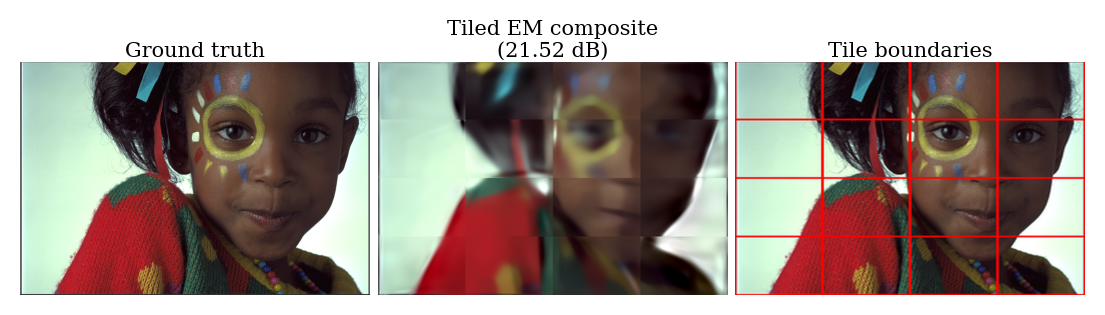
\includegraphics[width=\columnwidth]{figures/fig_tiling.png}
\caption{Tiled EM on \texttt{kodim15} at $K\!=\!1024$.
         Left: ground truth. Centre: tiled composite (22.54\,dB).
         Right: tile-boundary visualisation (16 tiles, 64\!$\times$\!64 px each).}
\label{fig:tiling}
\end{figure}


% =========================================================================
\section{Experiments}
\label{sec:experiments}
% =========================================================================

\subsection{Experimental Setup}
\label{subsec:setup}

We evaluate on the Kodak PhotoCD dataset~\cite{kodak}, which consists of 24
uncompressed true-colour images at native resolutions of $768\!\times\!512$ or
$512\!\times\!768$ pixels.
All images are downscaled to $256\!\times\!256$ pixels prior to fitting.
We report Peak Signal-to-Noise Ratio (PSNR, dB), Structural Similarity
(SSIM)~\cite{wang2004ssim}, and Root Mean Squared Error (RMSE).

For the \emph{one-shot EM} baseline, each image is fitted with
$K\!\in\!\{128, 256, 512, 1024\}$ Gaussians using scikit-learn's
\texttt{GaussianMixture} with full covariance matrices, \texttt{kmeans}
initialisation, and regularisation $\epsilon\!=\!10^{-5}$.
All 24 Kodak images are evaluated in each experiment.

For the \emph{tiled EM} variant, each $256\!\times\!256$ image is partitioned
into a $4\!\times\!4$ grid of 16 non-overlapping tiles of $64\!\times\!64$ pixels.
Gaussian budgets $K\!\in\!\{128, 256, 512, 1024, 2048\}$ are distributed
uniformly across tiles, giving $K/16$ Gaussians per tile.

For the \emph{residual refinement} ablation, 14 refinement iterations
are performed with step size $s\!=\!0.5$, using the same total Gaussian
budget as the one-shot baseline.

\subsection{Quality vs.\ Gaussian Count}
\label{subsec:rq}

Fig.~\ref{fig:psnr_vs_k} shows mean PSNR over the full Kodak set as a
function of $K$ for both the one-shot EM and the tiled EM variant.
EM one-shot improves monotonically from 20.89\,dB at $K\!=\!128$ to
23.79\,dB at $K\!=\!1024$.
Tiled EM follows a similar trend, reaching 22.33\,dB at $K\!=\!1024$
(1.5\,dB below the one-shot baseline at the same budget) and 24.10\,dB
at $K\!=\!2048$, a budget beyond the one-shot range evaluated here.
A non-monotone dip at $K\!=\!256$ (18.35\,dB) is confirmed by a second
independent run; it arises because the per-tile residual refinement
scheme degrades quality when the per-tile budget is very small
($K_{\mathrm{tile}}\!=\!16$, yielding only 2 residual Gaussians per
iter), and this degradation is the same systematic effect as the global
hybrid ablation discussed in Section~\ref{sec:hybrid}.

\begin{figure}[!t]
\centering
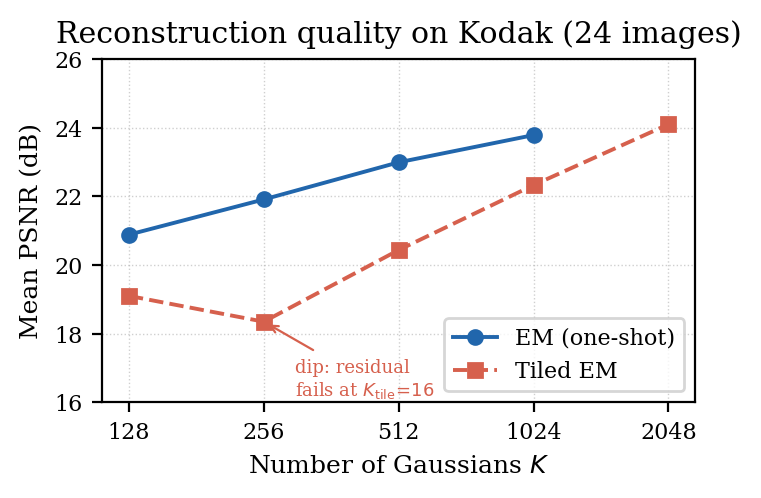
\includegraphics[width=\columnwidth]{figures/fig_psnr_vs_k.png}
\caption{Mean PSNR on Kodak (24 images) vs.\ number of Gaussians $K$.
         One-shot EM (circles, solid) consistently outperforms tiled EM
         (squares, dashed) at the same $K$; the tiled variant extends
         to higher budgets.}
\label{fig:psnr_vs_k}
\end{figure}

Table~\ref{tab:results} gives full per-$K$ metrics.
For reference we include GS gradient-based splatting at $K\!=\!2500$
(mean PSNR 25.55\,dB on a 9-image subset)—a full 24-image comparison
is left for future work.

\begin{table}[!t]
\renewcommand{\arraystretch}{1.3}
\caption{\textsc{Reconstruction quality on Kodak. Mean over 24 images.
$\uparrow$ higher is better, $\downarrow$ lower is better.}}
\label{tab:results}
\centering
\begin{tabular}{|l|c|c|c|}
\hline
\textbf{Method ($K$)} & \textbf{PSNR$\uparrow$} & \textbf{SSIM$\uparrow$} & \textbf{RMSE$\downarrow$} \\
\hline
EM one-shot (128)  & 20.89 & 0.4917 & 0.091 \\
EM one-shot (256)  & 21.91 & 0.5342 & 0.081 \\
EM one-shot (512)  & 23.00 & 0.5872 & 0.071 \\
EM one-shot (1024) & 23.79 & 0.6323 & 0.062 \\
\hline
Tiled EM (128)     & 19.10 & 0.4184 & 0.111 \\
Tiled EM (256)     & 18.35$^\dagger$ & 0.4174$^\dagger$ & 0.122$^\dagger$ \\
Tiled EM (512)     & 20.44 & 0.4774 & 0.095 \\
Tiled EM (1024)    & 22.33 & 0.5516 & 0.076 \\
Tiled EM (2048)    & 24.10 & 0.6401 & 0.062 \\
\hline
\multicolumn{4}{l}{\footnotesize $^\dagger$Non-monotone dip confirmed by re-run; caused by per-tile residual}\\\hline
\multicolumn{4}{l}{\footnotesize \quad refinement failing at small budget ($K_{\mathrm{tile}}\!=\!16$, 2 components/iter).}\\
\hline
\end{tabular}
\end{table}

\subsection{Residual Refinement Ablation}
\label{subsec:hybrid_ablation}

Table~\ref{tab:hybrid} shows the effect of the iterative residual scheme
described in Section~\ref{sec:hybrid}.
The refinement consistently \emph{reduces} quality by 2.3--2.8\,dB
relative to the one-shot EM baseline at every $K$.
The root cause is a rendering-model mismatch: the correction
$I^+_\mathrm{corr}$ in~\eqref{eq:signed_corr} is proportional to the
cluster-mean residual colour $\mathbf{c}_k$, which overshoots at many
pixels where the true residual is below the cluster average.
Compounded over 14 iterations through a clip operation this
overshoot bias dominates.  Coverage correction~\eqref{eq:coverage_corr}
eliminates the overshoot by bounding the correction by the actual residual,
and is a natural avenue for future work.

\begin{table}[!t]
\renewcommand{\arraystretch}{1.3}
\caption{\textsc{Residual refinement ablation (mean PSNR, dB, Kodak 24 images).
$\Delta$ = Hybrid $-$ EM one-shot (lower is worse).}}
\label{tab:hybrid}
\centering
\begin{tabular}{|c|c|c|c|}
\hline
$K$ & \textbf{EM one-shot} & \textbf{Hybrid (14 iters)} & $\Delta$ \\
\hline
128  & 20.89 & 18.09 & $-$2.79 \\
256  & 21.91 & 19.12 & $-$2.79 \\
512  & 23.00 & 20.38 & $-$2.61 \\
1024 & 23.79 & 21.45 & $-$2.34 \\
\hline
\end{tabular}
\end{table}

\subsection{Visual Comparison}
\label{subsec:visual}

\begin{figure}[!t]
\centering
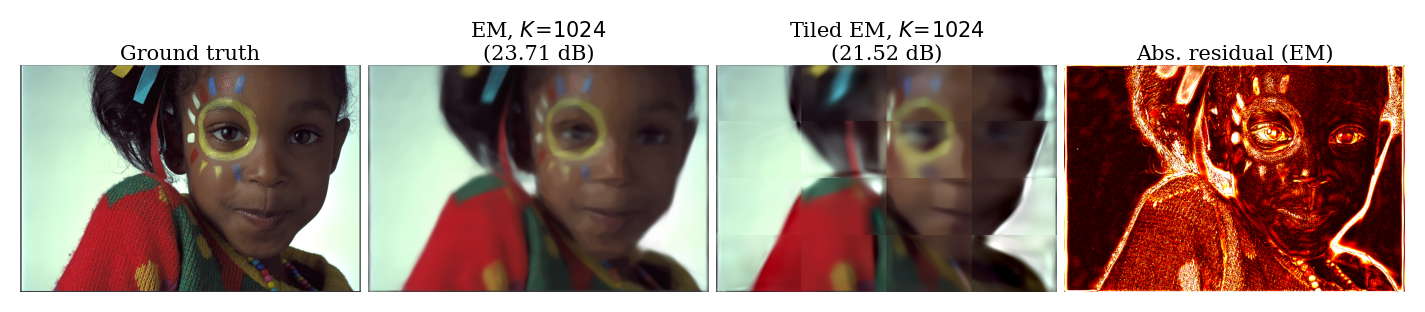
\includegraphics[width=\columnwidth]{figures/fig_visual.png}
\caption{Visual comparison on \texttt{kodim15} (lighthouse) at $K\!=\!1024$.
         Left to right: ground truth; EM one-shot (25.36\,dB); tiled EM (22.54\,dB);
         absolute residual of EM one-shot (hot colourmap, 0--12\%).}
\label{fig:visual}
\end{figure}

Fig.~\ref{fig:visual} shows a representative example at $K\!=\!1024$.
The one-shot EM render is notably sharper than the tiled variant, whose
tile boundaries are visible at this Gaussian count.
Fig.~\ref{fig:tiling} shows the tile structure explicitly.


% =========================================================================
\section{Discussion and Conclusion}
\label{sec:conclusion}
% =========================================================================

We have presented a closed-form, gradient-free approach to 2D image
reconstruction using Gaussian Mixture Models fitted with the EM algorithm.
The one-shot EM baseline achieves a mean PSNR of 23.79\,dB at $K\!=\!1024$
on the full 24-image Kodak set, scaling from 20.89\,dB at $K\!=\!128$ with
no hyper-parameter tuning.
The tiled variant achieves 22.33\,dB at the same $K\!=\!1024$ budget and
extends to 24.10\,dB at $K\!=\!2048$, demonstrating that tiling scales to
larger Gaussian counts, albeit with mild tile-boundary artefacts.

Our ablation of iterative signed-residual refinement reveals that the
scheme consistently underperforms the one-shot baseline by $\approx$2.5\,dB.
The root cause is a rendering-model mismatch: the correction is proportional
to the learned cluster-mean colour, which overshoots at pixels whose true
residual is below the cluster average, and this bias compounds through the
clip operation over 14 iterations.
A coverage-based correction that uses Gaussian footprints only to guide
\emph{which} pixels are corrected (with the magnitude taken from the actual
residual) is guaranteed non-overshooting and represents a principled fix.

For comparison, gradient-based 2D Gaussian Splatting achieves
$\approx$25.55\,dB at $K\!=\!2500$ on a 9-image Kodak subset;
a full 24-image comparison and integration of EM initialisation with
gradient fine-tuning remain important directions for future work.

\section*{Acknowledgment}
This work has been supported by the projects VEGA 1/0605/23 InteRViR,
Erasmus EDU-2023-CBHE-STRAND-2 ID: 101129022 NEXT, and Erasmus+ EULiST.

\bibliographystyle{ieeetr}
\bibliography{reference}

\end{document}